%%%%%%%%%%%%%%%%%%%%%%%%%%%%%%%%%%%%%%%%%%%%%%%%%%%%%%%%%%%%%%%%%%%%%%%%%%%%%%%%%%
\begin{frame}[fragile]\frametitle{}
\begin{center}
{\Large Rasa Chatbot Deployment}

\end{center}
\end{frame}

%%%%%%%%%%%%%%%%%%%%%%%%%%%%%%%%%%%%%%%%%%%%%%%%%%%%%%%%%%%
\begin{frame}[fragile]\frametitle{Slack Account Creation}
\begin{itemize}
\item First, create Slack Account, Workspace.
\item Create a new Workspace,https://slack.com/create#email, give email, verify it
\item Name of your company ``DataHacksConf2019'', thats the workspace name.
\item Project name ``rasachatbot'', thats the channel name.
\end{itemize}

\end{frame}

%%%%%%%%%%%%%%%%%%%%%%%%%%%%%%%%%%%%%%%%%%%%%%%%%%%%%%%%%%%
\begin{frame}[fragile]\frametitle{Slack App}
\begin{itemize}
\item Then, create a Slack App.
\item Visit https://api.slack.com/
\item Create a Slack app in ``RasaChatBotDemo'', 
\item Select ``DataHacksConf2019'' as Workspace
\end{itemize}

\begin{center}
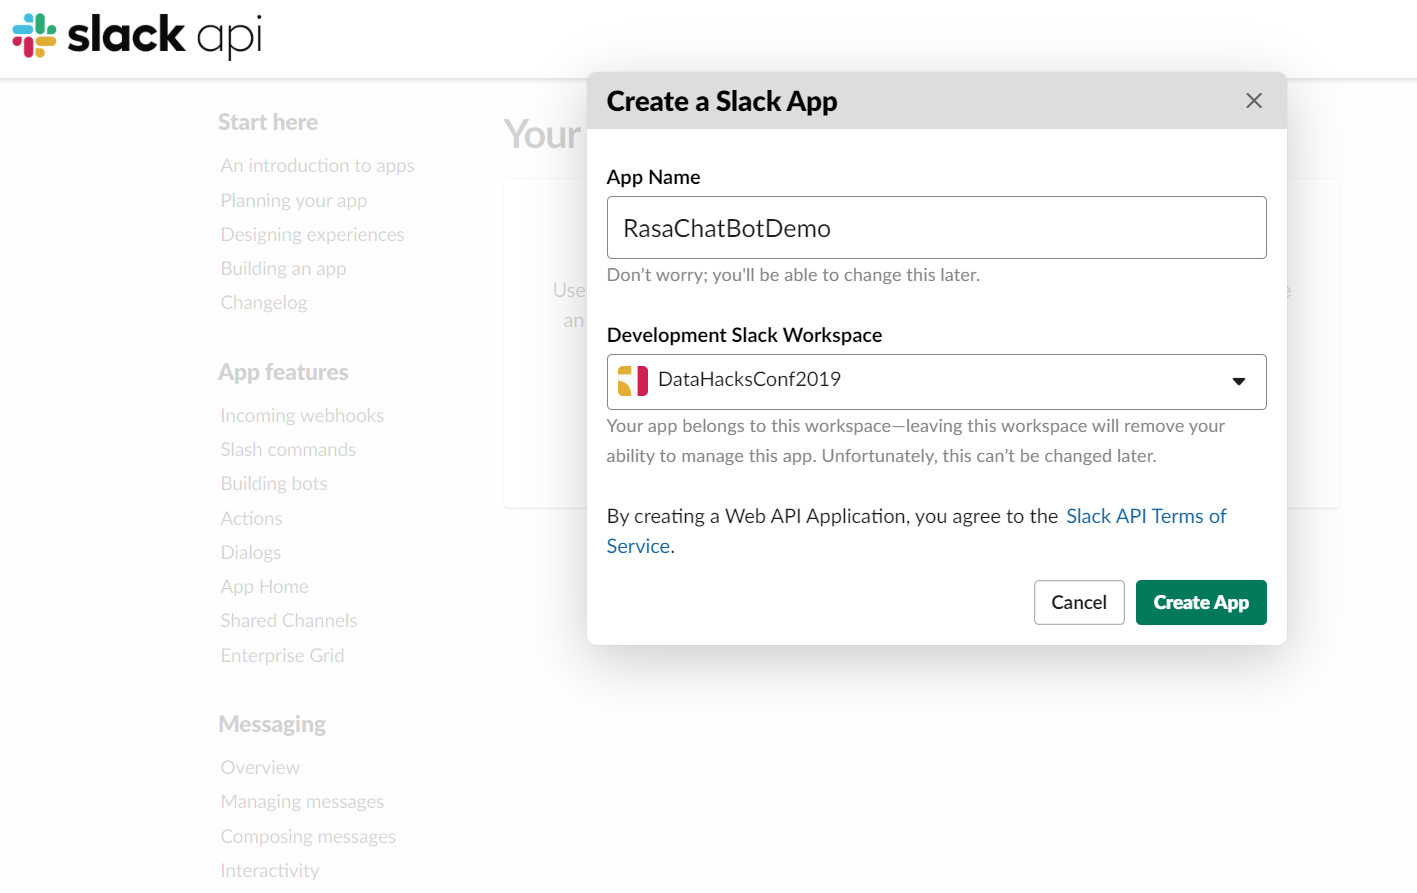
\includegraphics[width=0.5\linewidth]{rasa27}
\end{center}
\end{frame}

%%%%%%%%%%%%%%%%%%%%%%%%%%%%%%%%%%%%%%%%%%%%%%%%%%%%%%%%%%%
\begin{frame}[fragile]\frametitle{What's Next?}
How these modules work? 

Can dig deep, to find what different integrations are available \ldots

And build one \ldots

\end{frame}
